\documentclass[12pt, spanish]{article}
\usepackage[spanish]{babel}
\selectlanguage{spanish}
%\usepackage{natbib}
\usepackage{url}
\usepackage[utf8x]{inputenc}
\usepackage{graphicx}
\graphicspath{{images/}}
\usepackage{parskip}
\usepackage{fancyhdr}
\usepackage{vmargin}
\usepackage{multirow}
\usepackage{float}
\usepackage{chngpage}

\usepackage{amsfonts}

\usepackage{subcaption}

\usepackage{hyperref}
\usepackage[
    type={CC},
    modifier={by-nc-sa},
    version={4.0},
]{doclicense}

\hypersetup{
    colorlinks=true,
    linkcolor=blue,
    filecolor=magenta,      
    urlcolor=cyan,
}

% para codigo
\usepackage{listings}
\usepackage{xcolor}



%% configuración de listings

\definecolor{listing-background}{HTML}{F7F7F7}
\definecolor{listing-rule}{HTML}{B3B2B3}
\definecolor{listing-numbers}{HTML}{B3B2B3}
\definecolor{listing-text-color}{HTML}{000000}
\definecolor{listing-keyword}{HTML}{435489}
\definecolor{listing-identifier}{HTML}{435489}
\definecolor{listing-string}{HTML}{00999A}
\definecolor{listing-comment}{HTML}{8E8E8E}
\definecolor{listing-javadoc-comment}{HTML}{006CA9}

\lstdefinestyle{eisvogel_listing_style}{
  language         = python,
%$if(listings-disable-line-numbers)$
%  xleftmargin      = 0.6em,
%  framexleftmargin = 0.4em,
%$else$
  numbers          = left,
  xleftmargin      = 0em,
 framexleftmargin = 0em,
%$endif$
  backgroundcolor  = \color{listing-background},
  basicstyle       = \color{listing-text-color}\small\ttfamily{}\linespread{1.15}, % print whole listing small
  breaklines       = true,
  frame            = single,
  framesep         = 0.19em,
  rulecolor        = \color{listing-rule},
  frameround       = ffff,
  tabsize          = 4,
  numberstyle      = \color{listing-numbers},
  aboveskip        = 1.0em,
  belowskip        = 0.1em,
  abovecaptionskip = 0em,
  belowcaptionskip = 1.0em,
  keywordstyle     = \color{listing-keyword}\bfseries,
  classoffset      = 0,
  sensitive        = true,
  identifierstyle  = \color{listing-identifier},
  commentstyle     = \color{listing-comment},
  morecomment      = [s][\color{listing-javadoc-comment}]{/**}{*/},
  stringstyle      = \color{listing-string},
  showstringspaces = false,
  escapeinside     = {/*@}{@*/}, % Allow LaTeX inside these special comments
  literate         =
  {á}{{\'a}}1 {é}{{\'e}}1 {í}{{\'i}}1 {ó}{{\'o}}1 {ú}{{\'u}}1
  {Á}{{\'A}}1 {É}{{\'E}}1 {Í}{{\'I}}1 {Ó}{{\'O}}1 {Ú}{{\'U}}1
  {à}{{\`a}}1 {è}{{\'e}}1 {ì}{{\`i}}1 {ò}{{\`o}}1 {ù}{{\`u}}1
  {À}{{\`A}}1 {È}{{\'E}}1 {Ì}{{\`I}}1 {Ò}{{\`O}}1 {Ù}{{\`U}}1
  {ä}{{\"a}}1 {ë}{{\"e}}1 {ï}{{\"i}}1 {ö}{{\"o}}1 {ü}{{\"u}}1
  {Ä}{{\"A}}1 {Ë}{{\"E}}1 {Ï}{{\"I}}1 {Ö}{{\"O}}1 {Ü}{{\"U}}1
  {â}{{\^a}}1 {ê}{{\^e}}1 {î}{{\^i}}1 {ô}{{\^o}}1 {û}{{\^u}}1
  {Â}{{\^A}}1 {Ê}{{\^E}}1 {Î}{{\^I}}1 {Ô}{{\^O}}1 {Û}{{\^U}}1
  {œ}{{\oe}}1 {Œ}{{\OE}}1 {æ}{{\ae}}1 {Æ}{{\AE}}1 {ß}{{\ss}}1
  {ç}{{\c c}}1 {Ç}{{\c C}}1 {ø}{{\o}}1 {å}{{\r a}}1 {Å}{{\r A}}1
  {€}{{\EUR}}1 {£}{{\pounds}}1 {«}{{\guillemotleft}}1
  {»}{{\guillemotright}}1 {ñ}{{\~n}}1 {Ñ}{{\~N}}1 {¿}{{?`}}1
  {…}{{\ldots}}1 {≥}{{>=}}1 {≤}{{<=}}1 {„}{{\glqq}}1 {“}{{\grqq}}1
  {”}{{''}}1
}
\lstset{style=eisvogel_listing_style}


\usepackage[default]{sourcesanspro}

\setmarginsrb{2 cm}{1 cm}{2 cm}{2 cm}{1 cm}{1.5 cm}{1 cm}{1.5 cm}

\title{Práctica 2:\\
Desarrollo de un Sistema Experto  \hspace{0.05cm} }                           
\author{Antonio David Villegas Yeguas}                             
\date{\today}                                           

\renewcommand*\contentsname{hola}

\makeatletter
\let\thetitle\@title
\let\theauthor\@author
\let\thedate\@date
\makeatother

\pagestyle{fancy}
\fancyhf{}
\rhead{\theauthor}
\lhead{\thetitle}
\cfoot{\thepage}

\begin{document}

%%%%%%%%%%%%%%%%%%%%%%%%%%%%%%%%%%%%%%%%%%%%%%%%%%%%%%%%%%%%%%%%%%%%%%%%%%%%%%%%%%%%%%%%%

\begin{titlepage}
    \centering
    \vspace*{0.3 cm}
    
\includegraphics[scale = 0.50]{ugr.png}\\[0.7 cm]
    %\textsc{\LARGE Universidad de Granada}\\[2.0 cm]   
    \textsc{\large 3º CSI 2019/20 - Grupo 1}\\[0.5 cm]            
    \textsc{\large Grado en Ingeniería Informática}\\[0.5 cm]              
    \rule{\linewidth}{0.2 mm} \\[0.2 cm]
    { \huge \bfseries \thetitle}\\
    \rule{\linewidth}{0.2 mm} \\[1 cm]
    
    \begin{minipage}{0.4\textwidth}
        \begin{flushleft} \large
            \emph{Autor:}\\
            \theauthor\\ 
			 \emph{DNI:}\\
            77021623-M
            \end{flushleft}
            \end{minipage}~
            \begin{minipage}{0.4\textwidth}
            \begin{flushright} \large
            \emph{Asignatura: \\
            IC}   \\     
            \emph{Correo:}\\
            advy99@correo.ugr.es           
        \end{flushright}
    \end{minipage}\\[0.5cm]
  
    {\large \thedate}\\[0.5cm]
    %{\url{https://github.com/advy99/AA/}}
    {\doclicenseThis}
 	
    \vfill
    
\end{titlepage}

%%%%%%%%%%%%%%%%%%%%%%%%%%%%%%%%%%%%%%%%%%%%%%%%%%%%%%%%%%%%%%%%%%%%%%%%%%%%%%%%%%%%%%%%%

\tableofcontents
\pagebreak

%%%%%%%%%%%%%%%%%%%%%%%%%%%%%%%%%%%%%%%%%%%%%%%%%%%%%%%%%%%%%%%%%%%%%%%%%%%%%%%%%%%%%%%%%


\section{Funcionamiento del sistema experto.}

Tras cargar el fichero CLP de la práctica en CLIPS y ejecutarlo, como explico en el manual de uso, comenzará la ejecución del sistema experto.

Al principio encontraremos un menú que nos preguntará si queremos que se nos recomiende una rama o asignaturas.

Si seleccionamos la rama comenzarán las preguntas al igual que la práctica 1, pero para esta práctica se han corregidos errores de la primera práctica (ahora el sistema explica que razonamiento le ha llevado a escoger una rama y permite responder con información parcial cuando el usuario lo desee).


\begin{figure}[H]
	\centering
	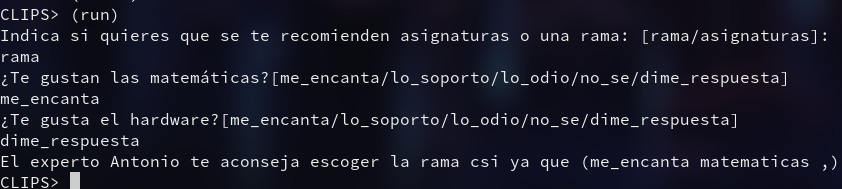
\includegraphics[scale=0.45]{ej_rama.png}
	\caption{Ejecución del sistema para recomendar una rama.}
	\label{rama}
\end{figure}


Si seleccionamos la segunda opción, asignaturas, el sistema pasará a preguntarnos entre que asignaturas queremos que se nos recomiende así como el número de créditos que queremos que se nos recomiende. Este número de créditos ha de ser múltiplo de 6 ya que una asignatura son 6 créditos y ha de ser mayor que 0 y menor o igual que 6 por el número de  asignaturas escogidas. Tras esto se nos realizarán preguntas para decidir que asignaturas recomendar.

Para este segundo apartado he decidido utilizar razonamiento por defecto, luego aunque no respondamos nada se nos recomendarán asignaturas. El procedimiento que sigue lo explicaré más adelante.

\begin{figure}[H]
	\centering
	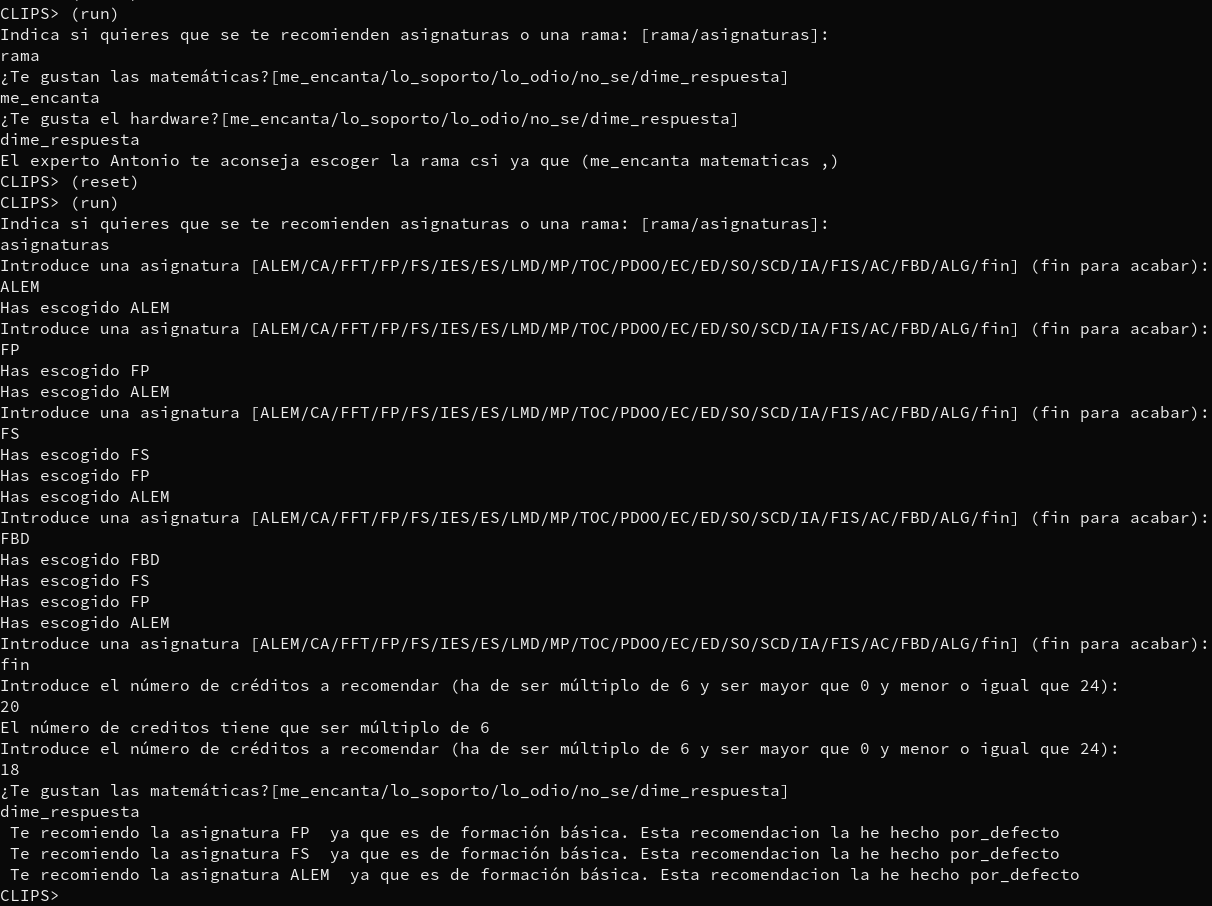
\includegraphics[scale=0.4]{ej_asig.png}
	\caption{Ejecución del sistema para recomendar asignaturas.}
	\label{ej_asig}
\end{figure}

Como podemos ver, al ejecutar el usuario sabe porque le recomendamos una asignatura, así como si la recomendación es por razonamiento por defecto y además puede solicitar en cualquier momento que se le haga la recomendación, aunque no responda todas las preguntas. 

\newpage

\section{Descripción del proceso seguido.}

En esta sección describiré el proceso seguido para desarrollar la base de conocimiento, la validación y la verificación del sistema a implementar en la práctica.

\subsection{Desarrollo de la base de conocimiento.}

Para el desarrollo de la base de conocimiento he tenido en cuenta la entrevista realizada en teoría como ejercicio y además información obtenida de la secretaría de la ETSIIT. Tras tener toda esta información la llevado a nuestro sistema usando CLIPS.

En esta práctica la base de conocimiento ha de tener información sobre las distintas asignaturas, así como si son de formación básica u obligatoria.

También tendremos en cuenta la rama de conocimiento y recomendaciones antes de cursar para realizar las recomendaciones, como por ejemplo si requieren una base matemática, de programación o de conocimientos de hardware.

Este conocimiento se ha implementado en el sistema como podemos ver en el código adjunto a esta memoria y también lo comentaré más adelante en la descripción del sistema.

\subsection{Validación y verificación del sistema.}

Para la verificación y validación de un sistema se han de seguir los siguientes pasos:

\begin{itemize}
	\item Verificar si el sistema es completo, preciso y consistente.
	\item Evaluar si el sistema cumple especificaciones del modelo de diseño.
	\item Diseñar un plan de validación aplicando metodologías apropiadas.
	\item Valorar en función de criterios de validación. Entre otros los requisitos funcionales definidos en la fase de identificación del problema.
\end{itemize}

\subsubsection{Verificación del sistema.}

Para verificar si el sistema es completo, preciso y consistente se siguen los siguientes pasos:

\begin{itemize}
	\item Construir el sistema correctamente.
	\item Descubrir y corregir errores en el SBC. En esta fase se analiza si es coherente, no válido.
	\item La verificación la realiza el ingeniero del conocimiento.
	\item Se ha de valorar que no hay conclusiones incoherentes, que las conclusiones son precisas y que no hay lagunas en la capacidad deductiva, es decir, es completo, el sistema siempre responde.
\end{itemize}

Como hemos visto la verificación del sistema la llevamos a cabo nosotros como ingenieros del conocimiento. En mi caso he comprobado que en la ejecución del sistema este siempre responde, aunque el usuario introduzca valores erróneos, o intente alguna opción compleja. 

En este análisis he comprobado que sea coherente, no válido, ya que como ingeniero del conocimiento he podido comprobar que obtengo respuestas por parte del sistema, que este no falla ni se queda colgado, sin embargo no soy capaz de saber si las respuestas dadas son las correctas acorde con el conocimiento del sistema ni si está razonando bien, esto último sería el proceso de validación, que pasaré a explicar en el siguiente punto.

\subsubsection{Validación del sistema.}

La validación no la realiza el ingeniero del conocimiento, si no que este utiliza al experto para comprobar que el sistema es correcto.

La validación comprobará los siguientes aspectos:

\begin{itemize}
	\item La comunicación con otros sistemas (transferencias) es adecuada.
	\item La interfaz es comprensible para el usuario.
	\item La explicación del razonamiento del sistema es suficiente.
	\item Cumple los requisitos de ejecución en tiempo real pedidos.
	\item Satisfacción y utilidad de los resultados finales e intermedios comparados con resultados conocidos, prestaciones de un experto u otros métodos.
\end{itemize}


Para comprobar todos estos aspectos he contactado con la persona que tomo el papel de experto en el ejercicio realizado en teoría y los resultados han sido positivos, ya que este considera que el sistema es fácil de usar y comprensible para el usuario porque en cada interacción el sistema especifica las posibles entradas, y aun así si existe algún error el sistema te avisa y es capaz de responder avisando al usuario y volviendo a realizar la pregunta.

El experto también me comento que tanto en la recomendación de rama y de asignaturas se realiza correctamente las explicaciones del razonamiento una vez ha dado respuesta y que tras varias pruebas con distintos casos que el conocía la respuestas son correctas.


\newpage

\section{Descripción del sistema.}

En este apartado explicaremos en profundidad el desarrollo del sistema, así como su estructura y explicación de la base de conocimiento.

\subsection{Variables de entrada del problema.}

Las variables de entrada del problema son la información que introduce el usuario a la base de conocimiento.

Al inicio el usuario ha de introducir que tipo de recomendación quiere, si quiere que se le recomienden ramas o asignaturas.

Una vez introduce ese conocimiento en la base de conocimiento el sistema le pide información acorde a este nuevo conocimiento.

En el caso de la recomendación de rama, el usuario introduce los siguientes hechos:

\begin{lstlisting}
(gusta ?cosa ?valor)
(trabajaria_en ?campo)
(es_trabajador ?valor)
\end{lstlisting}

Con el que representaremos que cosas le gustan o disgustan, en que campo trabajaría o si el usuario es trabajador.

Para la recomendación de asignaturas es necesaria más información, ya que el sistema ha de conocer sobre que asignaturas ha de hacer la recomendación, así como el número de créditos ha recomendar.

Utilizaremos los mismos hechos para representar los gustos del usuario, pero además utilizaremos los siguientes hechos para representar las asignaturas seleccionadas por el usuario, así como los créditos que quiere que le sean recomendados:

\begin{lstlisting}
(asignatura ?asig)
(creditos_asignar ?cred)
\end{lstlisting}


\newpage
\subsection{Variables de salida del problema.}

Las variables de salida del problema serán las recomendaciones que realice el sistema, ya sea la recomendación de una rama o la recomendación de asignaturas.

Los hechos que representan las recomendaciones en el caso de la rama son:

\begin{lstlisting}
(consejo ?rama ?apodo_experto)
(motivos ?motivos)
\end{lstlisting}

En el que el primer hecho representa la rama que finalmente aconseja el sistema y el segundo los motivos con los que ha razonado el sistema, basándose en las respuestas del usuario y la base de conocimiento.


En el caso de las asignaturas son:

\begin{lstlisting}
(recomendar ?asig ?recomendacion por_pregunta_respondida|por_defecto)
\end{lstlisting}

En este caso, al tener distintas asignaturas tendremos estos hechos para representar las que recomendamos, en las que vemos que contiene la asignatura, el motivo de la recomendación y si la recomendación se ha razonado defecto o porque se ha razonado tras información dada de un usuario.

\subsection{Conocimiento global del sistema.}

\subsection{Módulos desarrollados.}

\subsubsection{Estructura de los módulos.}

\subsubsection{Objetivo de cada módulo.}


\subsection{Hechos y reglas de cada módulo.}


\newpage

\section{Manual de uso del sistema.}

Para utilizar el sistema basta con cargar el fichero \texttt{p2.clp} adjunto en la entrega y realizar un reset y run en CLIPS.

\begin{lstlisting}
(load p2.clp)
(reset)
(run)
\end{lstlisting}

Tras esto el sistema mostrará un menú en el que debemos seleccionar si queremos que se nos recomiende una rama o asignaturas. Si escogemos rama se nos preguntará distintas cuestiones y nos recomendará una rama. También es posible que nos responda con información parcial. Ya hemos visto su funcionamiento en la figura \ref{rama}.


En el caso de seleccionar la recomendación de asignaturas, nos preguntará que asignaturas tenemos como candidatas y tenemos que responder con asignaturas que estén en la lista dada. Una vez escojamos asignaturas se nos preguntará el número de créditos que queremos que se nos recomiende, y este número ha de ser múltiplo de 6, al ser todas las asignaturas de 6 créditos. Tras esto pasará a realizarnos preguntas con las que razonará que asignaturas son más recomendadas, y en todo momento podemos pedir que se nos haga la recomendación, aunque tenga menos información. Este caso lo hemos visto en la figura \ref{ej_asig}.



\end{document}
